\documentclass[%
	paper=a4,
	fontsize=10pt,
	DIV11,BCOR10mm,
	numbers=noenddot,
	abstract=yes
]{scrartcl}

\usepackage[utf8]{inputenc}
\usepackage[english]{babel}
\usepackage[T1]{fontenc}
\usepackage{tgpagella}
\usepackage{microtype}


\usepackage{textcomp}
\usepackage{gensymb}


\usepackage{graphicx}
\graphicspath{{figures/}}


\usepackage{xfrac}
\usepackage{units}


\usepackage{amsmath}
\usepackage{amssymb}
\usepackage{amsthm}


\usepackage{mathtools}
\mathtoolsset{showonlyrefs=true}


\usepackage{scrhack} % for algorithm package
\usepackage[boxed]{algorithm}
\usepackage{algpseudocode}


\usepackage[
	style=alphabetic,
	bibstyle=alphabetic,
	maxbibnames=100,
	giveninits=true,
	useprefix=true,
	natbib=true,
	backend=biber]{biblatex}
\usepackage[strict=true]{csquotes}
\addbibresource{references.bib}


\usepackage{hyperref}
\hypersetup{
	%colorlinks,
	%citecolor=black,
	%filecolor=black,
	%linkcolor=black,
	%urlcolor=black,
	pdfauthor={Christoph Conrads},
	unicode=true,
}


% Make links jump to the beginning of figures and tables, not to the caption in
% them.
% This can also be fixed with the caption package.
\usepackage[all]{hypcap}



% bibliography with ngerman: @mastersthesis != Magisterarbeit
\DefineBibliographyStrings{english}{%
	mathesis = {MSc thesis},
}
\DefineBibliographyStrings{ngerman}{%
	mathesis = {Masterarbeit},
}



% Command definitions
\newcommand{\bigOh}[1]{\mathcal{O}(#1)}
\newcommand{\cond}[2][]{\kappa_{#1}(#2)}
\newcommand{\function}[1]{\textsc{#1}}
\newcommand{\almost}[1]{\widetilde{#1}}
\newcommand{\set}[1]{\mathcal{#1}}

\newcommand{\R}{\mathbb{R}}
\newcommand{\F}{\mathbb{C}}

\newcommand{\macheps}{\varepsilon}
\newcommand{\unitRO}{\mathbf{u}}
\newcommand{\tol}{\operatorname{tol}}

\DeclarePairedDelimiter\abs{\lvert}{\rvert}
\DeclarePairedDelimiter\norm{\lVert}{\rVert}
\DeclarePairedDelimiter\ceil{\lceil}{\rceil}

\DeclareMathOperator{\diag}{diag}
\DeclareMathOperator{\ran}{ran}
\DeclareMathOperator{\rank}{rank}
\DeclareMathOperator{\mathspan}{span}



\newtheorem{theorem}{Theorem}[section]
\newtheorem{corollary}{Corollary}[section]

\theoremstyle{definition}
\newtheorem{example}{Example}[section]
\newtheorem{definition}{Definition}[section]

% \bordermatrix with custom delimiters
% Source: Herbert Voß: "Math mode - v. 2.47", 2014, §5
\makeatletter
\newif\if@borderstar
\def\bordermatrix{\@ifnextchar*{%
    \@borderstartrue\@bordermatrix@i}{\@borderstarfalse\@bordermatrix@i*}%
}
\def\@bordermatrix@i*{\@ifnextchar[{\@bordermatrix@ii}{\@bordermatrix@ii[()]}}
\def\@bordermatrix@ii[#1]#2{%
\begingroup
  \m@th\@tempdima8.75\p@\setbox\z@\vbox{%
    \def\cr{\crcr\noalign{\kern 2\p@\global\let\cr\endline }}%
    \ialign {$##$\hfil\kern 2\p@\kern\@tempdima & \thinspace %
    \hfil $##$\hfil && \quad\hfil $##$\hfil\crcr\omit\strut %
    \hfil\crcr\noalign{\kern -\baselineskip}#2\crcr\omit %
    \strut\cr}}%
  \setbox\tw@\vbox{\unvcopy\z@\global\setbox\@ne\lastbox}%
  \setbox\tw@\hbox{\unhbox\@ne\unskip\global\setbox\@ne\lastbox}%
  \setbox\tw@\hbox{%
    $\kern\wd\@ne\kern -\@tempdima\left\@firstoftwo#1%
      \if@borderstar\kern2pt\else\kern -\wd\@ne\fi%
    \global\setbox\@ne\vbox{\box\@ne\if@borderstar\else\kern 2\p@\fi}%
    \vcenter{\if@borderstar\else\kern -\ht\@ne\fi%
      \unvbox\z@\kern-\if@borderstar2\fi\baselineskip}%
      \if@borderstar\kern-2\@tempdima\kern2\p@\else\,\fi\right\@secondoftwo#1 $%
  }\null \;\vbox{\kern\ht\@ne\box\tw@}%
\endgroup
}
\makeatother

\newcommand{\mybordermatrix}[1]{\bordermatrix[{[]}]{#1}}



\renewcommand{\algorithmicrequire}{\textbf{Input:}}
\renewcommand{\algorithmicensure}{\textbf{Output:}}
\algrenewcommand{\algorithmiccomment}[1]{\hskip1em\# #1}



\newcommand{\propername}[1]{\textsc{#1}}





\title{Computing with Chebychev Polynomials}
\author{Christoph Conrads {\small \url{https://christoph-conrads.name}}}



\begin{document}

\maketitle

\begin{center}
	\begin{minipage}{0.8\textwidth}
		This work is licensed under the Creative Commons Attribution-ShareAlike
		4.0 International License. To view a copy of this license, visit \\
		\url{http://creativecommons.org/licenses/by-sa/4.0/}
	\end{minipage}

	\vspace{1\baselineskip}

	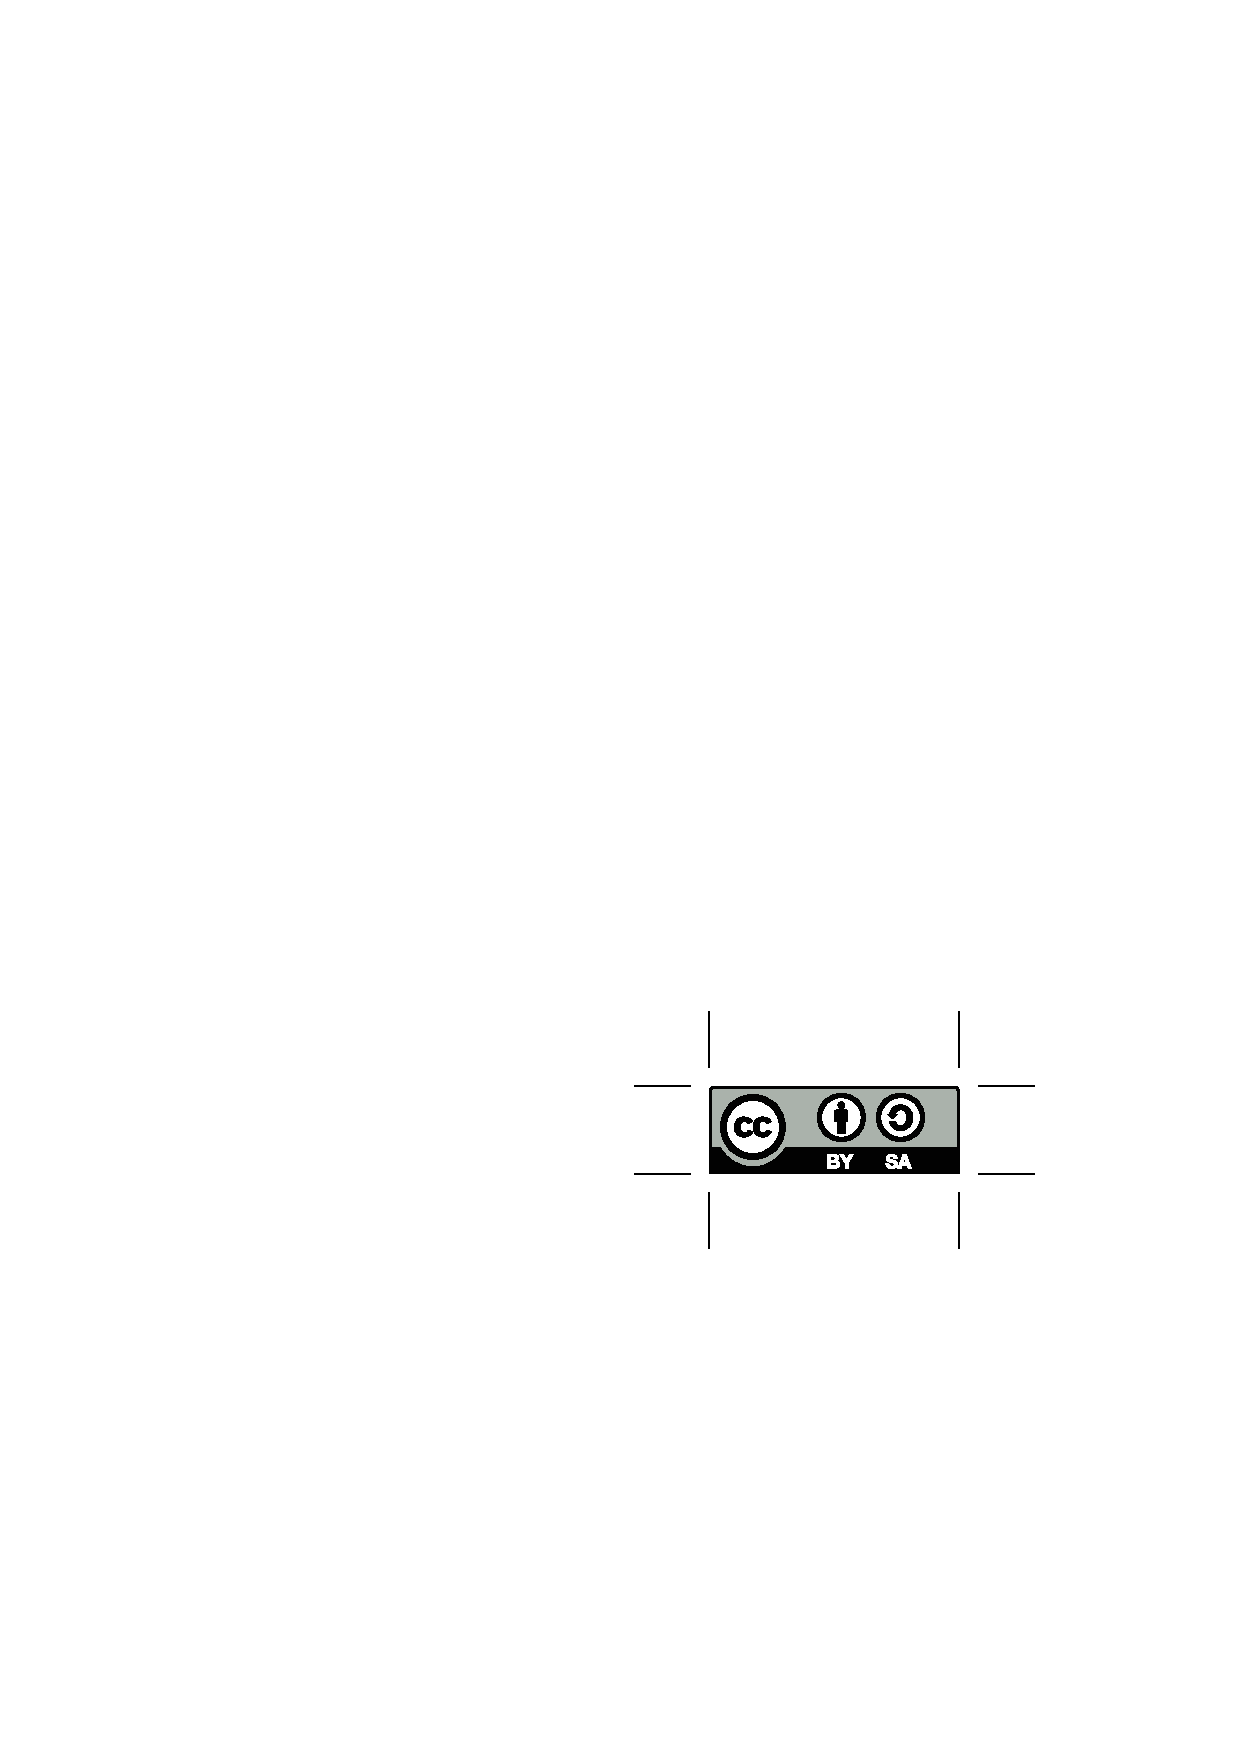
\includegraphics[width=8em]{creative-commons-by-sa}
\end{center}



\section{Introduction}

\begin{definition}[%
	{Chebychev polynomial of the first kind \cite[§4.4]{Saad2011}}]
	The \emph{Chebychev polynomial} $T_k(x): \R \rightarrow \R$ of the first
	kind is defined by
	\begin{align*}
		T_0(x) &= 0, \\
		T_1(x) &= t, \\
		T_{k+1}(x) &= 2x C_k(x) - C_{k-1}(x), k \geq 1.
	\end{align*}
\end{definition}

The following equality holds \cite[§4.4.1]{Saad2011}:
\[
	T_k(x) =
	\begin{dcases*}
		\cos[k \arccos(x)] & if $\abs{x} \leq 1$, \\
		\cosh[k \operatorname{arccosh}(x)] & otherwise,
	\end{dcases*}
\]
where $\cosh(x): \R \rightarrow \R$ is the hyperbolic cosine
\cite[§13.6]{Kreyszig2011}
\[ \cosh(x) = \sfrac{1}{2} (e^x + e^{-x}). \]
Chebychev polynomials are important in approximation theory.

\begin{theorem}[{\cite[Theorem~4.8]{Saad2011}}]
	Let $\alpha < \beta$, let $\gamma \not\in [\alpha, \beta]$. Let $c =
	\sfrac{1}{2} (\alpha + \beta)$, let $e = \sfrac{1}{2}(\beta - \alpha)$. Let
	$\mathbb{P}_k$ denote the set of all polynomials of degree $k$. Then the
	polynomial
	\[
		p_k^*(x) \coloneqq \frac%
			{T_k \left(\frac{x-c}{e}\right)}
			{T_k \left(\frac{\gamma-c}{e}\right)}
	\]
	is a solution of
	\[
		\min_{\substack{p \in \mathbb{P}_k \\ p(\gamma) = 1}}
		\max_{x \in [a,b]} \abs{p(x)}.
	\]
\end{theorem}

If $x$ is complex, a slightly weaker version of the theorem applies
\cite[Theorem 1]{Fischer1989}.

A Chebychev polynomial of degree $k$ has $k$ roots and all of them are in the
interval $[-1, +1]$.

\begin{theorem}
	Let $T_k(x)$ be a Chebychev polynomial of first kind. The roots $x_1, x_2,
	\dotsc, x_k$ of $T_k(x)$ are
	\[
		x_i = \cos \left( \frac{2i-1}{2k} \pi \right),
		i = 1, 2, \dotsc, k.
	\]
\end{theorem}

We can use the roots to factorize the Chebychev polynomial. Thus,
\[ T_k(x) = 2^{k-1} \mathop{\Pi}\limits_{i=1}^k (x - x_i). \]

In this text, we will use Chebychev polynomials in order to accelerate the
convergence of subspace iterations \cite[§5, §7.5]{Saad2011}. Let $A \in
\F^{n,n}$ have real eigenvalues and a full set of eigenvectors and consider we
seek the smallest eigenvalues of $A$. Then we can speed up the convergence of
inverse iteration by computing $p_k^*(A^{-1}) v$ instead of $A^{-1} v$, $v \in
\F^n$. Note that the multilevel eigensolver has always been using Chebychev
polynomials because the Cayley transformation $(x - c) / x$ is a Chebychev
polynomial with degree 1.



\section{Evaluating Chebychev Polynomials}

In this section we discuss the evaluation of matrix polynomials $p_k^*(A)$.
Specifically, we will consider the case where we use subspace iterations in
order to compute eigenvalues of the matrix pencil $K x = \lambda M x$, $K, M \in
F^{n,n}$, $K$, $M$ Hermitian positive definite. Then the matrix $A = M^{-1} K$
has the same eigenvalues as $(K, M)$ and we are interested in computing
$p_k^*(A)$.

It holds that
\[
	p_k^*(A) = \frac%
		{T_k \left(\frac{A-cI}{e}\right)}
		{T_k \left(\frac{\gamma-c}{e}\right)},
\]
where $\gamma$ is the smallest desired eigenvalue and $c+e < \gamma$, $[\alpha,
\beta]$ contains the set of unwanted eigenvalues, and $I$ is the identity
matrix. We can immediately drop the scaling factor $T_k(\sfrac{\gamma-c}{e})$
because the lengths of the calculated vectors are irrelevant (unless overflows
occur). Next, we have to ask ourselves how we can evaluate the Chebychev
polynomial $T_k(\sfrac{A-cI}{e})$. Using the definition of $T_k(x)$ involving
the trigonometric functions is not an option with (general) matrices but we
certainly, the recursive definition lends itself for this purpose:
\[
	p_k^*(A)v \approx
		2 \frac{A - cI}{e} \left[ T_{k-1}\left(\frac{A - cI}{e}\right)v \right]
		- T_{k-2}\left(\frac{A - cI}{e}\right)v, k \geq 2.
\]
Thus, we acquire Algorithm~\ref{algo:evaluate-polynomial}. Note the location of
the brackets makes a difference on a computer: $(A - cI) v$ instructs the
computer to calculate $A - cI$ before evaluating the matrix-vector product,
whereas $Av - cv$ contains a matrix-vector product and a vector-vector addition.
For optimal performance, we have to consider the following aspects:
\begin{itemize}
	\item Is $A$ sparse?
	\item If $A$ is sparse, how sparse is it?
	\item How many right-hand sides are there?
\end{itemize}
(See \cite[§2]{Davis2006} for basis of sparse matrix computations.) For example,
if $A$ is a sparse diagonal matrix and if $V \in \F^{n,m}$, $m \gg 1$, then it
is certainly faster to evaluate $(A - cI) V$ than $AV - cV$. The former involves
$n + nm$ operations whereas the latter requires $3nm$ flops. Finally, memory
usage is dependent on brackets as well, e.\,g.,
\[ v_{i+1} = \sfrac{2}{e} (A - cI) v_i - v_{i-1} \]
requires storage for $A$, $A - cI$, $v_{i-1}$, $v_i$, and $v_{i+1}$, whereas
\[ v_{i+1} = \sfrac{2}{e} A v_i - \sfrac{2c}{e} v_i - v_{i-1} \]
stores $A$ and two vectors; linear algebra software like \propername{Lapack}
provides operations $w \coloneqq \alpha A v + \beta w$, $\alpha, \beta \in \F$,
so we might perform the following operations when minimizing the need for
memory:
\begin{itemize}
	\item Compute $v_{i-1} \coloneqq \sfrac{2}{e} A v_i - v_{i-1}$,
	\item compute $v_{i-1} \coloneqq v_{i-1} - \sfrac{2c}{e} v_i$, and
	\item rename $v_{i-1}$ to $v_{i+1}$.
\end{itemize}

Alternatively, we can use the fact that we know the roots of the Chebychev
polynomial:
\begin{align*}
	v_1 &= \sfrac{1}{e} (A - x_1 I) v, \\
	v_{i+1} &= \sfrac{1}{e} (A - x_{i+1} I) v_i, \, i = 1, 2, \dotsc, k.
\end{align*}

\begin{algorithm}
	\begin{algorithmic}
		\Function{evaluate-polynomial}{$c, e, A, v$}
			\State $v_0 \gets 0 \in \F^n$
			\State $v_1 \gets \sfrac{1}{e} (A - cI) v$

			\Statex
			\For{$i = 1, 2, \dotsc, k-1$}
				\State $v_{i+1} = \sfrac{2}{e} (A - cI) v_i - v_{i-1}$
			\EndFor

			\Statex
			\State \textbf{return} $v_k$
		\EndFunction
	\end{algorithmic}
	\caption{A simple iterative method for evaluating Chebychev polynomials
	$p_k^*(A) v$.}
	\label{algo:evaluate-polynomial}
\end{algorithm}

Next, let us consider the problem of computing the smallest eigenvalues of $A =
M^{-1} K$. Again, there are computational trade-offs and here we present some
possibilities:
\begin{itemize}
	\item $[(M^{-1} K) - cI] v$: matrix-matrix solve, matrix-matrix addition,
		matrix-vector multiplication;
	\item $(M^{-1} K)v - cv$: matrix-matrix solve, matrix-vector multiplication,
		vector-vector addition;
	\item $M^{-1} [(K - c M) v]$: matrix-matrix addition, matrix-vector
		multiplication, matrix-vector solve.
\end{itemize}
With many right-hand sides and sparse matrices $K$ and $M$, evaluating $M^{-1}
[(K - cM) V]$ is the most efficient ordering. Furthermore, this scheme only
needs to store two dense matrices, namely $V$ and $(K - cM) V$.



\section{Numerical Experiments}

Scaled Chebychev polynomials were implemented in DCGeig in commit 06a2, July 22,
2016. They were replaced with unscaled polynomials using the polynomial's roots
in commit 6885, July 24, 2016. Note other changes were commit in between so in
order to evaluate the effect of commit 6885, you need to compare with the
results of commit 1e13, July 24, 2016. There is a small, discernible
difference, e.\,g., for the matrix s3dkq4m2 the solver reduced from
\unit[5471]{s} to \unit[5441]{s} wall-clock time (\unit[9951]{s} vs
\unit[9909]{s} CPU time).



\printbibliography

\end{document}
